\section{Constructing the MQL algebra tree}
\label{sect:impl:construct_mql}
MQL queries are constructed as trees, where each node represents an operator. Each node is an instance of an
operator class, and may contain a list of child operators and a list of parameters. The trees are constructed
bottom-up while parsing the abstract syntax tree corresponding to a XQuery query.

\subsection{Operators and parameters}
\begin{figure}[!htp]
\begin{center}
  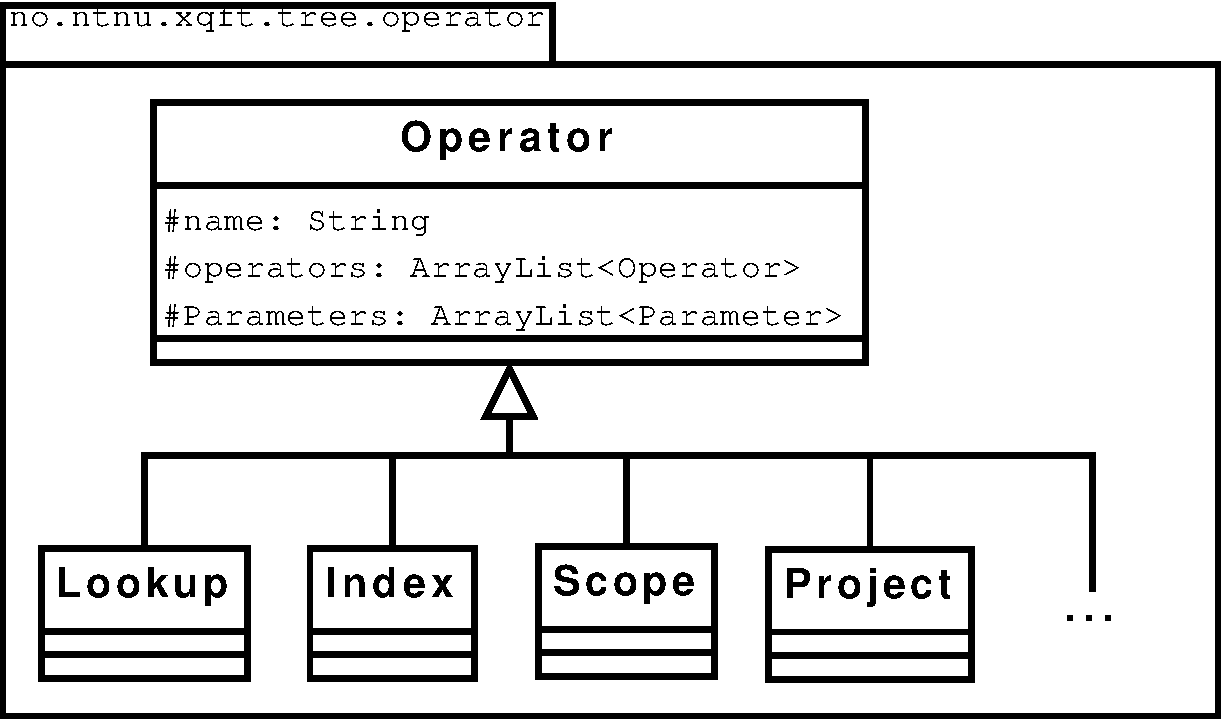
\includegraphics[scale=0.5]{diagrams/mql_operator_uml}
  \caption{Simplified class diagram of MQL operators}
  \label{fig:impl:mql_op_uml}
\end{center}
\end{figure}
The operators modeled in the implementation correspond to the operators
described in Section \ref{sect:method:marsOperators}. A simplified class
diagram is shown in Figure \ref{fig:impl:mql_op_uml}. Converting an operator to a string is in most cases
handled by the default fallback in the \texttt{Operator} class, where the string generated will be on the form:
\begin{Verbatim}
operator_name(param1, param2, ..., paramN; 
    operator1;
    operator2; 
    ...; 
    operatorM)
\end{Verbatim}

Constructing such a string for the complete query tree is achieved by calling \texttt{toPrettyString(0)} on the
root node. The parameter to the method specifies the initial indentation.

\begin{figure}[!htp]
\begin{center}
  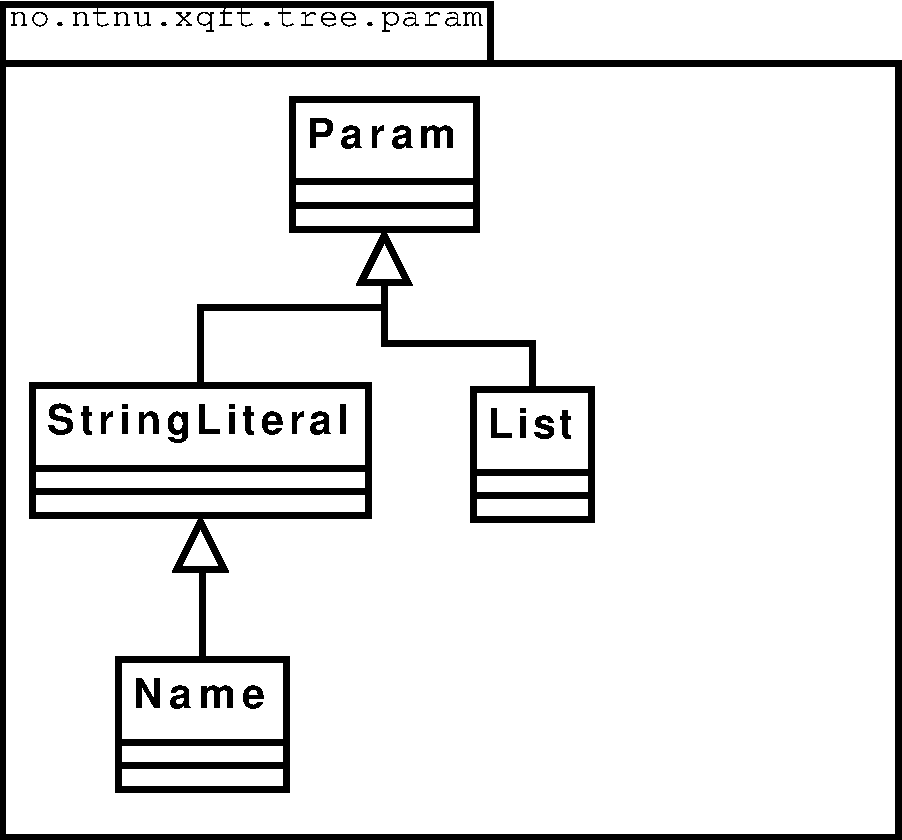
\includegraphics[scale=0.5]{diagrams/mql_param_uml}
  \caption{Class diagram of MQL parameters}
  \label{fig:impl:mql_param_uml}
\end{center}
\end{figure}

MQL parameters (as described in \ref{sect:method:mql:concepts}) are modeled as
seen in Figure \ref{fig:impl:mql_param_uml}. Parameters require no complex
structure, and are only created and added to operators as needed.

\subsection{Usage}
The operator classes are designed to be intuitive and simple to use. Figure
\ref{fig:impl:mql_op_ex1_java} shows one example where a simple operator tree
is built and converted to an MQL query string. The result can be seen in Figure \ref{fig:impl:mql_op_ex1_mql}).

%\usepackage{graphics} is needed for \includegraphics
\begin{figure}[htp]
\begin{center}
  \begin{Verbatim}
Lookup lookup = new Lookup("Death in the clouds");
Scope scope = new Scope("/books/book/title", lookup);
Project project = new Project("author", scope);
System.out.println(project.toPrettyString(0));
  \end{Verbatim}
  \caption{Example java code to construct a MQL operator tree}
  \label{fig:impl:mql_op_ex1_java}
\end{center}
\end{figure}

\begin{figure}[htp]
\begin{center}
  \begin{Verbatim}
project(author;
  scope(/books/book/title;
    lookup("Death in the clouds")))
  \end{Verbatim}
  \caption{Resulting MQL query string from example in figure
  \ref{fig:impl:mql_op_ex1_java}}
  \label{fig:impl:mql_op_ex1_mql}
\end{center}
\end{figure}
